\documentclass{examen}

\begin{document}
\modulo{Lenguajes de marcas -- PARTE ESCRITA}

\pregunta{Crear en HTML un formulario como el mostrado en la figura}{2}
\begin{figure}[h]
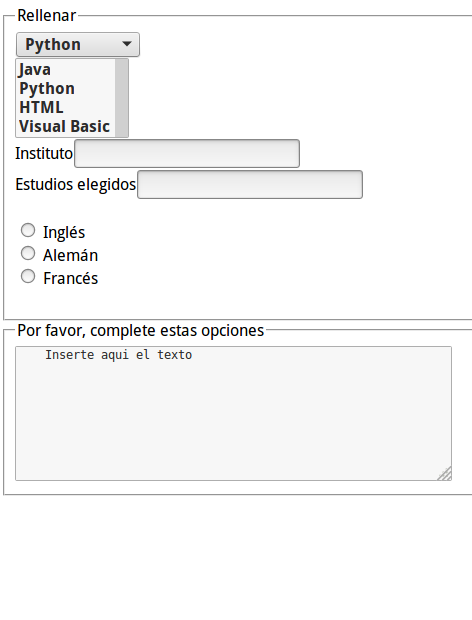
\includegraphics[scale=0.5]{examen-img/foto_formulario_11.png}
\end{figure}
\break

\pregunta{Crear un fichero de esquema XML que permita validar un fichero XML como el mostrado al final y para el cual se han definido las siguientes reglas}{3}
\begin{itemize}
\item{    El elemento ra�z se llama documentos.}
\item{    Dentro de �l puede haber uno o m�s elementos documento.}
\item{    Un documento debe empezar con un elemento creador, que siempre es una cadena de texto o empezar
por un elemento vac�o llamado {\tt creadordesconocido}}
\item{    Un documento siempre debe llevar una fecha de creaci�n. La fecha debe llevar siempre un atributo
llamado {\tt formato} que lleva dentro una cadena de texto.}
\item{    Un documento siempre debe llevar un elemento llamado {\tt uso}. El uso siempre ser� una
de estas tres cadenas de texto: {\tt Privado.} {\tt P�blico} o {\tt Desconocido}     }
\item{    Todo documento debe llevar un elemento {\tt paginas} que debe llevar dentro un n�mero entero positivo.}
\end{itemize}


\begin{verbatim}
<documentos>
    <documento>
        <creador>Juan Sanchez</creador>
        <fecha_creacion formato="ESP">20-Dic-2016</fecha_creacion>
        <uso>Privado</uso>
        <paginas>240</paginas>
    </documento>
    <documento>
        <creadordesconocido/>
        <fecha_creacion formato="ENG">12-21-2012</fecha_creacion>
        <uso>P�blico</uso>
        <paginas>240</paginas>
    </documento>
</documentos>

\end{verbatim}
\end{document}
